\documentclass[12pt]{report}
\usepackage[utf8]{inputenc}
\usepackage[russian]{babel}
%\usepackage[14pt]{extsizes}
\usepackage{listings}

% Для листинга кода:
\lstset{ %
language=python,                 % выбор языка для подсветки (здесь это С)
basicstyle=\small\sffamily, % размер и начертание шрифта для подсветки кода
numbers=left,               % где поставить нумерацию строк (слева\справа)
numberstyle=\tiny,           % размер шрифта для номеров строк
stepnumber=1,                   % размер шага между двумя номерами строк
numbersep=5pt,                % как далеко отстоят номера строк от подсвечиваемого кода
showspaces=false,            % показывать или нет пробелы специальными отступами
showstringspaces=false,      % показывать или нет пробелы в строках
showtabs=false,             % показывать или нет табуляцию в строках
frame=single,              % рисовать рамку вокруг кода
tabsize=2,                 % размер табуляции по умолчанию равен 2 пробелам
captionpos=t,              % позиция заголовка вверху [t] или внизу [b] 
breaklines=true,           % автоматически переносить строки (да\нет)
breakatwhitespace=false, % переносить строки только если есть пробел
escapeinside={\#*}{*)}   % если нужно добавить комментарии в коде
}

% Для измененных титулов глав:
\usepackage{titlesec, blindtext, color} % подключаем нужные пакеты
\definecolor{gray75}{gray}{0.75} % определяем цвет
\newcommand{\hsp}{\hspace{20pt}} % длина линии в 20pt
% titleformat определяет стиль
\titleformat{\chapter}[hang]{\Huge\bfseries}{\thechapter\hsp\textcolor{gray75}{|}\hsp}{0pt}{\Huge\bfseries}


% plot
\usepackage{pgfplots}
\usepackage{filecontents}
\usetikzlibrary{datavisualization}
\usetikzlibrary{datavisualization.formats.functions}
\begin{filecontents}{Levenshtein(Matrix).dat}
2 0.0000727
3 0.0000120
4 0.0000190
5 0.0000266
6 0.0000368
7 0.0000499
8 0.0000603
9 0.0000753
\end{filecontents}

\begin{filecontents}{Levenshtein(Recursion).dat}
2 0.0000723
3 0.0000340
4 0.0001767
5 0.0009067
6 0.0049724
7 0.0312771
8 0.1437498
9 0.7829850
\end{filecontents}

\begin{filecontents}{Damerau-Levenshtein(Matrix).dat}
2 0.0000738
3 0.0000129
4 0.0000203
5 0.0000297
6 0.0000449
7 0.0000601
8 0.0000685
9 0.0000848
\end{filecontents}

\begin{filecontents}{Damerau-Levenshtein(Recursion).dat}
2 0.0000803
3 0.0000377
4 0.0001908
5 0.0010294
6 0.0057501
7 0.0304088
8 0.1575722
9 0.8673832
\end{filecontents}

\begin{filecontents}{Levenshtein.dat}
10 0.00009
20 0.00034
30 0.00071
40 0.00128
50 0.00206
100 0.00777
200 0.03242
\end{filecontents}

\begin{filecontents}{Damerau-Levenshtein.dat}
10 0.00010
20 0.00040
30 0.00086
40 0.00155
50 0.00242
100 0.00980
200 0.04048
\end{filecontents}


\begin{document}
 
%\def\chaptername{} % убирает "Глава"
\begin{titlepage}
	\centering
	{\scshape\LARGE МГТУ им. Баумана \par}
	\vspace{3cm}
	{\scshape\Large Лабораторная работа №1\par}
	\vspace{0.5cm}	
	{\scshape\Large По курсу: "Анализ алгоритмов"\par}
	\vspace{1.5cm}
	{\huge\bfseries Расстояние Левенштейна\par}
	\vspace{2cm}
	\Large Работу выполнил: студент группы ИУ7-53Б Наместник Анастасия\par
	\vspace{0.5cm}
	\LargeПреподаватели:  Волкова Л.Л., Строганов Ю.В.\par

	\vfill
	\large \textit {Москва, 2020} \par
\end{titlepage}

\tableofcontents

\newpage
\chapter*{Введение}
\addcontentsline{toc}{chapter}{Введение}

\textbf{            Расстояние Левенштейна (редакционное расстояние)} -  минимальное количество односимвольных операций (а именно вставки, удаления, замены), необходимых для превращения одной последовательности символов в другую.\\

\textit{Редакционным предписанием} называется последовательность действий, необходимых для получения из первой строки второй кратчайшим образом.

Расстояние Левенштейна на практике используется для решения таких задач, как:

\begin{itemize}
	\item  исправление ошибок в слове (в поисковых системах, базах данных, при вводе текста, при автоматическом распознавании отсканированного текста или речи);
	\item сравнение текстовых файлов утилитой diff и ей подобными. Здесь роль «символов» играют строки, а роль «строк» — файлы;
	\item сравнение генов, хромосом и белков  в биоинформатике.
\end{itemize}

Целью данной лабораторной работы является изучение, реализация и сравнительный анализ алгоритмов
Левенштейна и Дамерау-Левенштейна. 

В данной лабораторной работе требуется решить четыре задачи.
\begin{enumerate}
  	\item Изучить алгоритмы Левенштейна и Дамерау-Левенштейна нахождения расстояния между строками.
	\item Получить практические навыкы реализации указанных алгоритмов: двух алгоритмов в матричной версии и двух алгоритмов в рекурсивной версии.
	\item Сделать сравнительный анализ по затрачиваемым памяти и времени.
	\item Описать и обосновать полученные результаты в отчете о выполненной лабораторно
работе.
\end{enumerate}


\chapter{Аналитическая часть}
Задача по нахождению расстояния Левенштейна заключается в поиске минимального количества операций вставки/удаления/замены для превращения одной строки в другую.
 
\textbf{Обозначение операций, применимых к символам:} 
\begin{enumerate}
  	\item D (англ. delete) — удаление;
	\item I (англ. insert) — вставка;
	\item R (replace) — замена;
	\item M (match) - совпадение.
\end{enumerate}

\section{Расстояние Левенштейна}
Пусть $S_{1}$ и $S_{2}$ — две строки (длиной M и N соответственно) над некоторым алфавитом, тогда расстояние Левенштейна можно подсчитать по рекуррентной формуле \ref{eq:ref1}:

\begin{equation}
D(i,j) = \left\{ \begin{array}{ll}
 0, & \textrm{$i = 0, j = 0$}\\
 i, & \textrm{$j = 0, i > 0$}\\
 j, & \textrm{$i = 0, j > 0$}\\
min(\\
D(i,j-1)+1,\\
D(i-1, j) +1, &\textrm{$j>0, i>0$}\\
D(i-1, j-1) + m(S_{1}[i], S_{2}[j])\\
\label{eq:ref1}
),
  \end{array} \right.
\end{equation}

где $m(a,b)$ равна нулю, если $a=b$ и единице в противном случае; $min\{\,a,b,c\}$ возвращает наименьший из аргументов.\\

\section{Расстояние Дамерау-Левенштейна}
При нахождении расстояния Дамерау — Левенштейна добавляется операция транспозиции (перестановки соседних символов).  

Расстояние Дамерау-Левенштейна вычисляется по рекуррентной формуле \ref{eq:ref2}:
\begin{equation}
D(i,j) = \left\{ \begin{array}{ll}
 0, & \textrm{$i = 0, j = 0$}\\
 i, & \textrm{$j = 0, i > 0$}\\
 j, & \textrm{$i = 0, j > 0$}\\
min(\\
D(i,j-1)+1,\\
D(i-1, j) +1, &\textrm{$j>0, i>0$}\\
D(i-1, j-1) + m(S_{1}[i], S_{2}[j])\\
\left[
\begin{array}{c}
D(i-2, j-2) + 1, $ если $i,j>1$ и $a_{i} = b_{j-1}, a_{i-1}=b_{j},\\
\infty $ , иначе )$
\end{array} \right.
\label{eq:ref2}\\
  \end{array} \right.
\end{equation}

Каждый рекурсивный вызов соответствует одному из случаев:
\begin{itemize}
	\item $d_{a, b}$(i - 1, j) + 1 соответствует удалению символа (из a в b);
	\item $d_{a, b}$(i, j - 1) + 1 соответствует вставке (из a в b);
	\item $d_{a, b}$(i - 1, j - 1) + 1 соответствие или несоответствие, в зависимости от совпадения символов;
	\item $d_{a, b}$(i - 2, j - 2) + 1 в случае перестановки двух последовательных символов,  +inf иначе.
\end{itemize}

\section{Вывод}
В аналитической части были получены краткие теоретические сведения о поиске расстояния Левенштейна и об аналогичном алгоритме, отличающемся на одну операцию, - алгоритм поиска расстояния Дамерау-Левенштейна, а также были приведены рекуррентные формулы обоих алгоритмов.

\chapter{Конструкторская часть}
Ниже представлены схемы рассматриваемых алгоритмов.

\begin{figure}[ht!]
	\centering{
		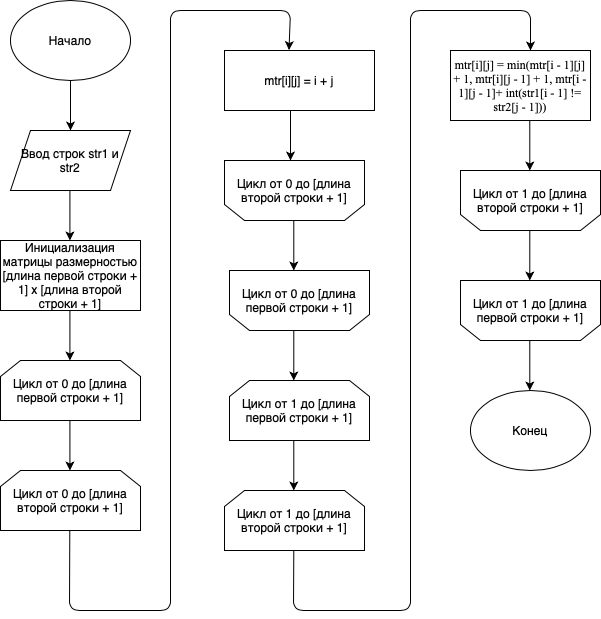
\includegraphics[width=0.6\textwidth]{schema/Lev.png}
		\caption{Схема алгоритма Левенштейна (матрица)}
		\label{fg:ref3}}
\end{figure}

\begin{figure}[ht!]
	\centering{
		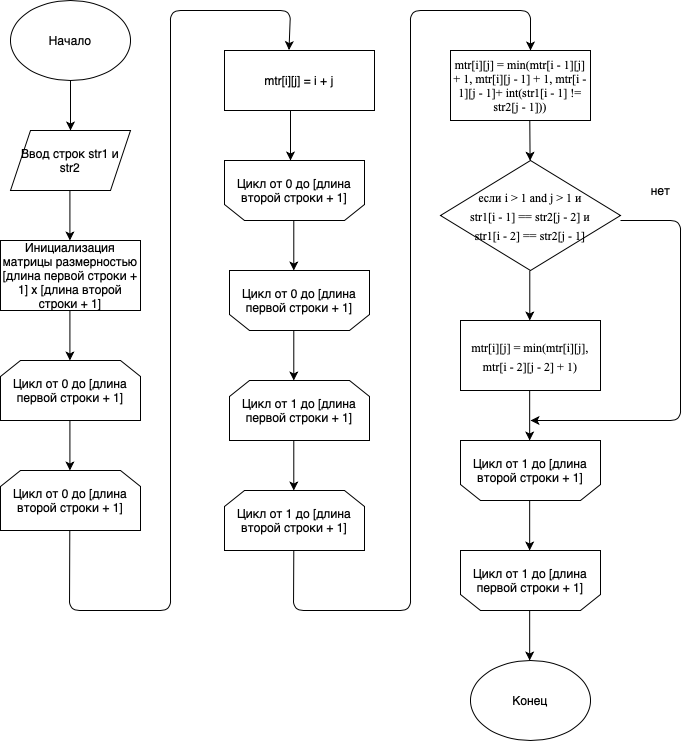
\includegraphics[width=0.6\textwidth]{schema/DLev.png}
		\caption{Схема алгоритма Дамерау-Левенштейна (матрица)}
		\label{fg:ref4}}
\end{figure}

\begin{figure}[ht!]
	\centering{
		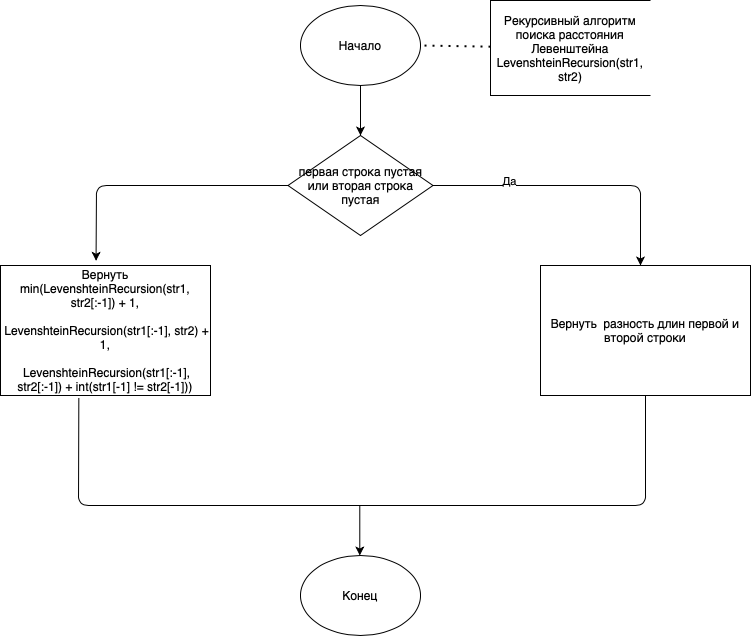
\includegraphics[width=0.6\textwidth]{schema/LevRec.png}
		\caption{Схема алгоритма Левенштейна (рекурсия)}
		\label{fg:ref5}}
\end{figure}

\begin{figure}[ht!]
	\centering{
		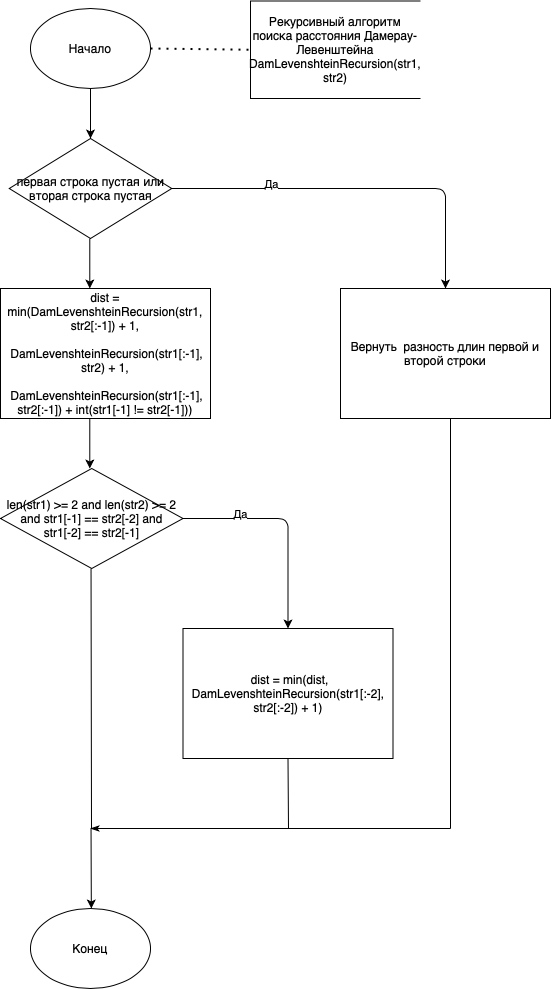
\includegraphics[width=0.6\textwidth]{schema/DLevRec.png}
		\caption{Схема алгоритма Дамерау-Левенштейна (рекурсия)}
		\label{fg:ref6}}
\end{figure}

\section{Вывод}
В данном разделе были рассмотрены схемы четырех алгоритмов: алгоритмы поиска расстояния Левенштейна и Дамерау-Левенштейна с матричной и рекурсивной реализацией. Из полученных данных можно визуально оценить емкость каждого из алгоритмов и предположить, что рекурсивный подход к расстоянию Левенштейна наименее затратный, с точки зрения написания кода.

\chapter{Технологическая часть}
\section{Выбор ЯП}
В данной лабораторной работе использовался язык программирования - python (3.8.3) \cite{bib1} в целях упрощения работы со структурами и визуализацией данных сравнительных анализов, а также из-за наличия опыта работы с данным ЯП. В качестве интегрированной среды разработки использовался интерпретатор python - IDLE  \cite{bib2}. Для замеров процедурного времени использовалась функция process\_time() библиотеки time \cite{bib3}. В качестве инструмента измерения затраченной памяти использовалась библиотека memory\_profiler \cite{bib4}.

\section{Сведения о модулях программы}
Программа состоит из следующих модулей:
\begin{itemize}
	\item editorial\_distance.py - главный файл программы;
	\item test.py - файл с тестами;
	\item time.py - файл с замерами временнных характеристик.
\end{itemize}

\begin{lstlisting}[label=some-code,caption=Подпрограмма поиска расстояния Левенштейна с помощью таблицы]
def LevenshteinMatrix(str1, str2):
    n = len(str1) + 1
    m = len(str2) + 1
    mtr = [[(i + j) for j in range(m)] for i in range(n)]

    for i in range(1, n):
        for j in range(1, m):
            mtr[i][j] = min(mtr[i - 1][j] + 1, mtr[i][j - 1] + 1,
                            mtr[i - 1][j - 1] + int(str1[i - 1] != str2[j - 1]))
    return mtr
\end{lstlisting}

\begin{lstlisting}[label=some-code,caption=Подпрограмма поиска расстояния Левенштейна рекурентно]
def LevenshteinRecursion(str1, str2):
    if not str1:
        return len(str2)
    if not str2:
        return len(str1)
    return min(LevenshteinRecursion(str1, str2[:-1]) + 1,
               LevenshteinRecursion(str1[:-1], str2) + 1,
               LevenshteinRecursion(str1[:-1], str2[:-1]) + int(str1[-1] != str2[-1]))\end{lstlisting}

\begin{lstlisting}[label=some-code,caption=Подпрограмма поиска расстояния Дамерау-Левенштейна с помощью таблицы]
def DamLevenshteinMatrix(str1, str2):
    n = len(str1) + 1
    m = len(str2) + 1
    mtr = [[(i + j) for j in range(m)] for i in range(n)]

    for i in range(1, n):
        for j in range(1, m):
            mtr[i][j] = min(mtr[i - 1][j] + 1, mtr[i][j - 1] + 1,
                            mtr[i - 1][j - 1] + int(str1[i - 1] != str2[j - 1]))
            if i > 1 and j > 1 and str1[i - 1] == str2[j - 2] and str1[i - 2] == str2[j - 1]:
                mtr[i][j] = min(mtr[i][j], mtr[i - 2][j - 2] + 1)

    return mtr
\end{lstlisting}

\begin{lstlisting}[label=some-code,caption=Подпрограмма поиска расстояния Дамерау-Левенштейна рекурентно]
def DamLevenshteinRecursion(str1, str2):
    if not str1:
        return len(str2)
    if not str2:
        return len(str1)

    dist = min(DamLevenshteinRecursion(str1, str2[:-1]) + 1,
               DamLevenshteinRecursion(str1[:-1], str2) + 1,
               DamLevenshteinRecursion(str1[:-1], str2[:-1]) + int(str1[-1] != str2[-1]))
    if (len(str1) >= 2 and len(str2) >= 2 and str1[-1] == str2[-2] and str1[-2] == str2[-1]):
        dist = min(dist, DamLevenshteinRecursion(str1[:-2], str2[:-2]) + 1)
    return dist
\end{lstlisting}

\section{Тесты}

Было реализовано несколько видов тестов:
\begin{itemize}
	\item сравнение результата матричного и рекурсивного алгоритмов поиска расстояния Левенштейна и Дамерау-Левенштейна при заданном количестве тестов и количестве символов в строке, которая генерируется с помощью отдельной процедуры;
	\item проверка работы обоих алгоритмов с пустой строкой;
	\item проверка работы обоих алгоритмов, если строки равны.
\end{itemize}
\begin{lstlisting}[label=randStr,caption=Функция генерации строки заданной длины]
def StringGen(strlen):
    l = string.ascii_lowercase
    return ''.join(random.choice(l) for i in range(strlen))
\end{lstlisting}

\begin{lstlisting}[label=randStr,caption=Функция проверки работы алгоритмов при пустой строке]
def EmptyString(func):
    strlen = int(input("Enter the string length: "))
    s = StringGen(strlen)

    if func == LevenshteinMatrix or func == DamLevenshteinMatrix:
        mtr = func(s, "")
        return int(mtr[len(mtr) - 1][len(mtr[len(mtr) - 1]) - 1] == len(s))
    dist = func(s, "")
    return int(dist == len(s))
\end{lstlisting}

\begin{lstlisting}[label=randStr,caption=Функция проверки работы алгоритмов при одинаковых строках]
def EqualStrings(func):
    strlen = int(input("Enter the string length: "))
    s = StringGen(strlen)

    if func == LevenshteinMatrix or func == DamLevenshteinMatrix:
        mtr = func(s, s)
        return int(mtr[len(mtr) - 1][len(mtr[len(mtr) - 1]) - 1] == 0)
    dist = func(s, s)
    return int(dist == 0)
\end{lstlisting}

\begin{lstlisting}[label=randStr,caption=Функция проверки работы матричного и рекурсивного алгоритма поиска расстояния Левенштейна]
def cmp_Lev_matrix_recursion():

    print("\033[33m{:<}\n".format(
        "*****Levenshtein distance (matrix/recursion)*****"))
    print("\033[0m")

    t = int(input("Enter the number of tests: "))

    for i in range(t):
        count = 0

        strlen = int(input("Enter the string length: "))
        str1, str2 = StringGen(strlen), StringGen(strlen)
        mtr, dist = LevenshteinMatrix(
            str1, str2), LevenshteinRecursion(str1, str2)
        count += int(mtr[len(mtr) - 1][len(mtr[len(mtr) - 1]) - 1] == dist)
        PrintRes(count)
\end{lstlisting}

\begin{lstlisting}[label=randStr,caption=Функция проверки работы матричного и рекурсивного алгоритма поиска расстояния Дамерау-Левенштейна]
def cmp_DamLev_matrix_recursion():

    print("\033[33m{:<}\n".format(
        "*****Damerau-Levenshtein distance (matrix/recursion)*****"))
    print("\033[0m")

    t = int(input("Enter the number of tests: "))

    for i in range(t):
        count = 0

        strlen = int(input("Enter the string length: "))
        str1, str2 = StringGen(strlen), StringGen(strlen)
        mtr, dist = DamLevenshteinMatrix(
            str1, str2), DamLevenshteinRecursion(str1, str2)
        count += int(mtr[len(mtr) - 1][len(mtr[len(mtr) - 1]) - 1] == dist)
        PrintRes(count)
\end{lstlisting}

\section{Вывод}
В технологической части были представлены модули программы, листинги кода и тестов к программе, а также обусловлен выбор языка программирования и приведены использовавшиеся в ходе работы инструменты.


\chapter{Исследовательская часть}

\section{Результат замеров времени выполнения всех алгоритмов} 

Сравним временные показатели работы каждого из рассматриваемых четырех алгоритмов при длине строки от 2 до 9 символов. Для этого установим количество итераций (повторений вызова процедуры) iter и воспользуемся библиотекой time для замера времени выполнения каждого алгоритма по iter раз. Возьмем iter = 50, а длины строк равными [2, 3, 4, 5, 6, 7, 8, 9]. Время выполнения алгоритмов со строками небольшой длины довольно мало, поэтому чтобы оценить его, следует взять среднее арифметическое от времени, за которое процедура отработает установленные iter раз. Результат приведен в таблице \ref{table:ref1}:
\begin{table}[ht]
	\centering
	\caption{Сравнительная таблица времени выполнения всех алгоритмов}
	\begin{tabular}{|c c c c c|}
		\hline
		Длина строки & Лев(м) & Лев(р) & Дам-Лев(м) & Дам-Лев(р) \\ [0.5ex] 
 		\hline\hline
		2 & 0.0000727 & 0.0000723 & 0.0000738 & 0.0000803\\
 		\hline
 		3 & 0.0000120 & 0.0000340 & 0.0000129 & 0.0000377\\
 		\hline
 		4 & 0.0000190 & 0.0001767 & 0.0000203 & 0.0001908\\
 		\hline
		5 & 0.0000266 & 0.0009067 & 0.0000297 & 0.0010294\\
		\hline
		6 & 0.0000368 & 0.0049724 & 0.0000449 & 0.0057501\\
		\hline
		7 & 0.0000499 & 0.0312771 & 0.0000601 & 0.0304088\\
		\hline
		8 & 0.0000603 & 0.1437498 & 0.0000685 & 0.1575722\\
		\hline
		9 & 0.0000753 & 0.7829850 & 0.0000848 & 0.8673832\\
		\hline
	\end{tabular}
	\label{table:ref1}
\end{table} 

\begin{figure}[ht!]
	\centering{
		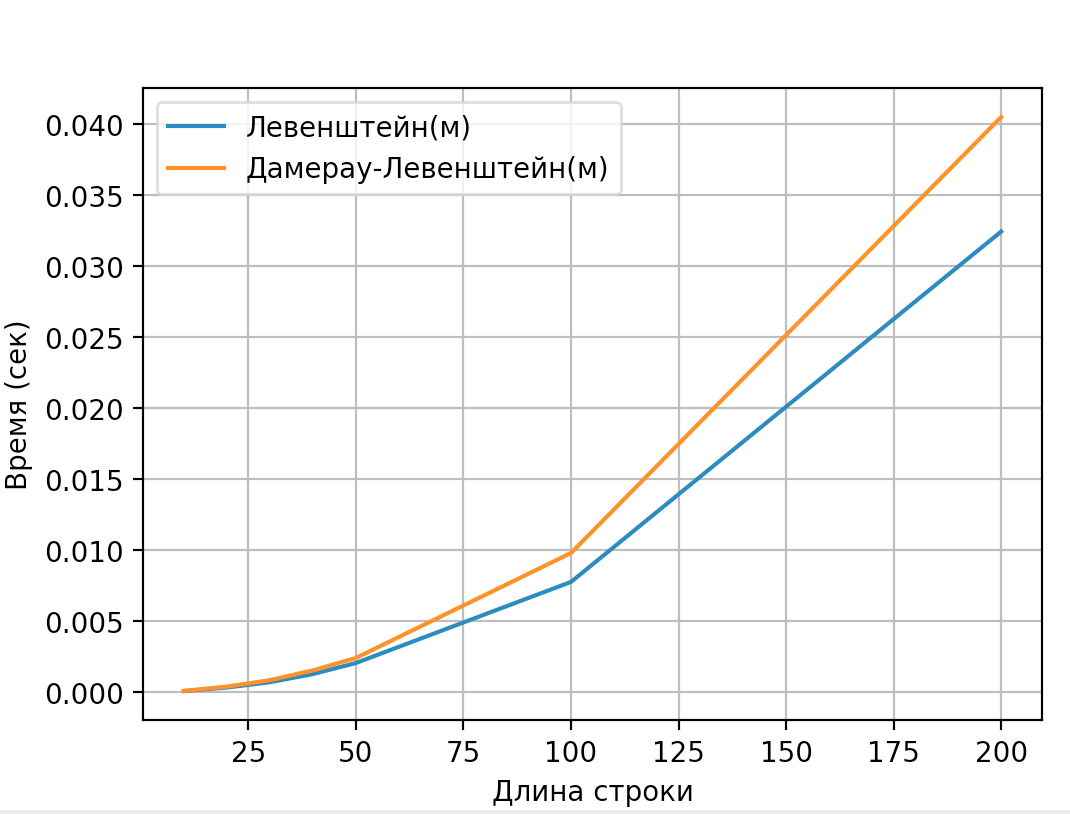
\includegraphics[width=0.6\textwidth]{pics/Lev-DLev(m).png}
		\caption{Сравнение времени выполнения всех алгоритмов} 
		\label{fg:ref1}}
\end{figure}


\par

Из рисунка \ref{fg:ref1} следует, что рекурсивные алгоритмы Левенштейна и Дамерау-Левенштейна значительно уступают по времени выполнения соответствующим матричным алгоритмам, причем уже при длине строки в 9 символов рекурсивный алгоритм Дамерау-Левенштейна начинает работать медленнее алгоритма Левенштейна, что обусловливается дополнительной операцией транспозиции. Однако, можно заметить, что при таких длинах строк затруднительно сделать сравнительный анализ матричных алгоритмов, для этого потребуются более длинные строки и большее количество повторений процедур.

\section{Результат замеров времени выполнения матричных алгоритмов} 

Для того чтобы получить примерное время работы матричных алгоритмов Левенштейна и Дамерау-Левенштейна, аналогично предыдущему эксперименту, возбмем фиксированные длины строк [10, 20, 30, 40, 50, 100, 200] и количество итераций iter = 500. Суммарное время выполнения процедуры, запущенной iter раз, нужно разделить на iter. Результат представлен в сравнительной таблице \ref{table:ref2}.

\begin{table}[ht]
	\centering
	\caption{Сравнительная таблица времени выполнения алгоритмов Левенштейна и Дамерау-Левенштейна в матричной реализации}
	\begin{tabular}{|c c c c c|}
		\hline
		\hline
		String length & Левенштейн & Дамерау-Левенштейн \\ [0.5ex] 
 		\hline\hline
		10 & 0.00009 & 0.00010\\
 		\hline
 		20 & 0.00034 & 0.00040\\
 		\hline
 		30 & 0.00071 & 0.00086\\
 		\hline
		40 & 0.00128 & 0.00155\\
		\hline
		50 & 0.00206 & 0.00242\\
		\hline
		100 & 0.00777 & 0.00980\\
		\hline
		200 & 0.03242 & 0.04048\\
		\hline
		\end{tabular}
	\label{table:ref2}
\end{table} 

\begin{figure}[ht!]
	\centering{
		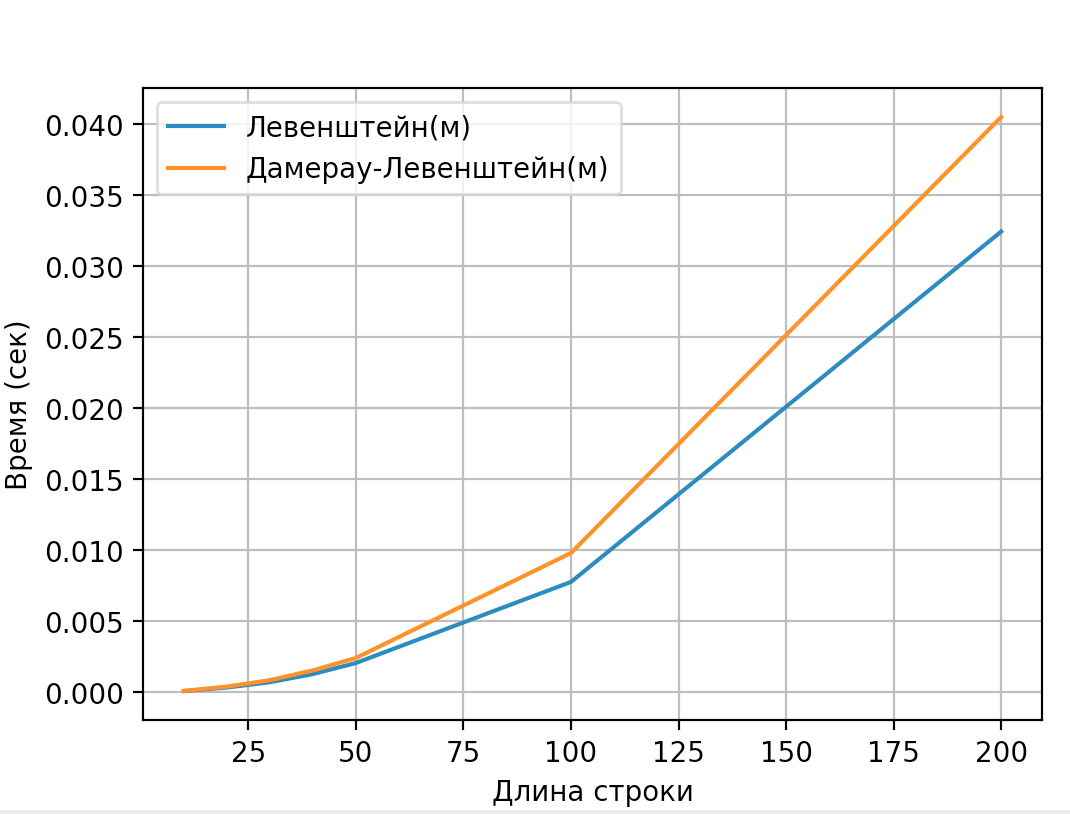
\includegraphics[width=0.6\textwidth]{pics/Lev-DLev(m).png}
		\caption{Сравнение времени выполнения алгоритмов Левенштейна и Дамерау-Левенштейна в матричной реализации} 
		\label{fg:ref2}}
\end{figure}


Анализ рисунка \ref{fg:ref2}, отражающего зависимость времени выполнения матричных алгоритмов Левенштейна и Дамерау-Левенштейна от длины строки, показывает, что при относительно малых длинах строк различия во времени незначительны, однако при длине 100 символов и больше алгоритм Дамерау-Левенштейна 
работает уже заметно медленнее, и при 200 символах его скорость становится ниже почти в 1.3 раза. Как уже было сказано, такое расхождение во времени объясняется четвертой операцией (транспозиция), утяжеляющей данный алгоритм.

\section{Анализ затрачиваемой памяти}

Память, затрачиваемая на реализацию матричный алгоритмов Левенштейна и Дамерау-Левенштейна, представляет собой произведение размерности матрицы и количество байт, занимаемых типом integer (в языке программирования python - 28 байт). Рекурсивные алгоритмы избыточны за счет повторных вызовов, уже при длине строки в 2 символа количество вызовов рекурсии составит 18 раз. Каждый вызов занимает 32 Мегабайта. Таким образом, рекурсивный подход займет 32x18 = 576 Мегабайт.

\section{Вывод}
Из полученных экспериментальным путем данных очевидно считать алгоритм поиска расстояния Левенштейна, реализованный с помощью матрицы, наиболее оптимальным как с точки зрения временных характеристик, так и относительно затрачиваемой памяти. В то же время результаты сравнительных анализов показывают, что рекуррентный алгоритм поиска расстояния Дамерау-Левенштейна является самым медленным и самым емким по занимаемым ресурсам памяти.

\chapter*{Заключение}
\addcontentsline{toc}{chapter}{Заключение}
В ходе лабораторной работы были реализованы и проанализированы алгоритмы поиска редакционного расстояния Левенштейна и Дамерау-Левенштейна, изучены особенности и отличия данных алгоритмов, а также способы их реализации: матричный, рекурсивный. В целях оценки эффективности алгоритмов, был проведён сравнительный анализ временных характеристик с учетом строк малых и больших длин, который позволил установить, что алгоритмы, реализованные с помощью рекуррентных формул, работают значительно медленнее матричных из-за многочисленных вызовов процедуры с повторяющимися параметрами, а также то, что в самих рекурсивных алгоритмах расхождение во времени заметно уже к длине слова в 9 символов (формула Дамерау-Левенштейна содержит дополнительную операцию). При сравнении матричных алгоритмов было выяснено, что скорость работы алгоритма Дамерау-Левенштейна становится ниже при длине слова в 100 символов, где алгоритм Левенштейна почти в 1.3 раза быстрее. Таким образом, алгоритм Дамерау-Левенштейна и при матричной, и при рекурсивной реализации работает медленнее алгоритма Левенштейна за счёт четвёртой операции - транспозиции. Также можно выделить недостаток рекурсивной реализации у обоих алгоритмов - наличие повторных вызовов, что снижает эффективность такого подхода. Из вышеизложенного справедливо утверждать, что матричный алгоритм поиска расстояния Левенштейна является самым выгодным по затрачиваемым на его выполнение ресурсам, а рекуррентный алгоритм поиска расстояния Дамерау-Левенштейна, наоборот, самый медленный и емкий из всех рассмотренных алгоритмов.

\bibliographystyle{gost780u}
\bibliography{books}



\end{document}